\documentclass{article}

\usepackage[%
    left=0.5in,%
    right=0.5in,%
    top=0.5in,%
    bottom=0.5in,%
]{geometry}%
\usepackage{minitoc}
\usepackage{multicol}
\usepackage{graphicx}
\usepackage{fixltx2e}
\usepackage{listings}
\usepackage{color}
\usepackage{hyperref}
    \hypersetup{ colorlinks = true, linkcolor = blue }
\usepackage{blindtext}
\definecolor{lightgray}{gray}{0.9}
\graphicspath{ {./} }

\newcommand{\inlinecode}[2]{\colorbox{lightgray}{\lstinline
[language=#1]$#2$}}
\newcommand{\worddef}[1]{\hyperref[sec:reference]{\textit{#1}}}

\begin{document}

\tableofcontents

\newpage

\section{Crytography}

\section{Encryption}
\begin{itemize}
  \item Encryption: We encode a message such that only authorised users may read it
  \item Cipher: takes a string of plaintext, and converts it into a string of ciphertext
  \item Encryption can provide: Confidentiality, Integrity, Authenticity
\end{itemize}

\section{Notation}
\begin{itemize}
  \item A \textit{cipher} converts a plaintext message \textbf{M} into a \textit{ciphertext} \textbf{C} under the control of a key \textbf{K} 
  \item C is \textbf{not a secret}, but without knowledge of the key, it should be impossible to \textbf{reconstruct} M
  \item Comes in two forms: \textit{Symmetric} – same key for encryption / decryption. \textit{Asymmetric} – separate keys
\end{itemize}

\section{The One Time Pad}
\begin{flushleft}
Using XOR to encrypt the message:
\begin{itemize}
  \item Use a key that’s the \textbf{same length} as the message 
  \item XOR each message bit with each key bit
  \item Any possible plaintext can be recovered depending on the key
  \item This is an example where $M = C - K mod 26$
\end{itemize}
\end{flushleft}
\begin{center}
  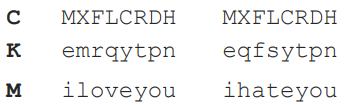
\includegraphics[scale=0.5]{one_time-pad.png}
\end{center}
\begin{flushleft}
It is an impractical method because:
\end{flushleft}
\begin{itemize}
  \item A 1GB file would need a 1GB key! 
  \item How are we transporting these keys? Or storing them? 
  \item If you ever \textbf{reuse a key}, the entire cipher is broken
\end{itemize}

\section{Modern Stream Ciphers}
\begin{itemize}
  \item Modern stream ciphers use an initial seed key to generate an infinite pseudorandom keystream 
  \item The message and keystream are usually combined using XOR - ⊕ - which is reversible if applied twice
  \item Common to seed an initial state using a key, then update this state for as long as needed
\end{itemize}

\begin{center}
  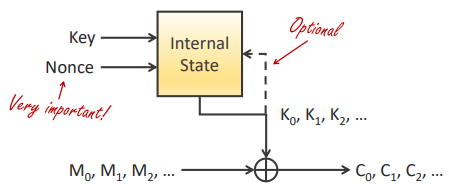
\includegraphics[scale=0.5]{modern_cyphers.png}
\end{center}

\subsection{ChaCha20}

\begin{center}
  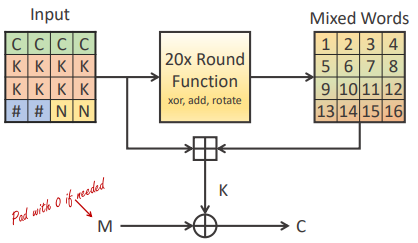
\includegraphics[scale=0.5]{chacha.png}
\end{center}
\begin{itemize}
  \item ChaCha performs 20 rounds: alternates Column and Diagonal Rounds, each round is 4 quarter rounds
  \item It's fast, because ChaCha20 is based on ARX (Addition-Rotation-XOR) which are \textbf{CPU friendly instruction}
\end{itemize}

\subsection{Advantages of Stream Ciphers}
\begin{itemize}
  \item Encrypting long continuous streams, possibly of unknown length. E.g. GSM mobile communications 
  \item Extremely \textbf{fast with a low memory footprint}, ideal for low-power devices 
  \item If designed well, can seek to any location in the steam. E.g. Streaming video with DRM
\end{itemize}

\subsection{Vulnerabilities}
\begin{itemize}
  \item Stream ciphers give us confidentiality, but not integrity 
  \item We must include another mechanism
\end{itemize}

\section{Hash functions}
\begin{itemize}
  \item A hash function is any function that can be used to map data of arbitrary size to data of a \textbf{fixed size}
  \item Hash functions are used everywhere. Message authentication, integrity, passwords etc
  \item Usually hash functions iteratively jumble blocks of a message after another 
  \item Once all the message is gone, we read the current hash. 
  \item The initial hash is usually defined in the spec
\end{itemize}

\subsection{Strong Hash Functions}
\begin{itemize}
  \item The output must be indistinguishable from random noise 
  \item Bit changes must diffused through the entire output. A small change to a message should change the hash value so extensively that the new hash value appears uncorrelated with the old hash value
  \item For a hash function to be useful, we need it to have some important properties:
  \begin{itemize}
    \item One-way: Given h(M), we can’t calculate M easily
    \item Weak collision resistance: Given M and h(M), we cannot find some M’ s.t. h(M) = h(M’)
    \item Strong collision resistance: We can’t find some message pair M ≠ M’ s.t. h(M) = h(M’)
  \end{itemize}
\end{itemize}

\subsection{The Birthday Attack}
\begin{itemize}
  \item \textbf{The Birthday Paradox}: concerns the probability that, in a set of n randomly chosen people, some pair of them will have the same birthday
  \item The output of the hash must be long enough to avoid a birthday attack.
  \item Given a hash function outputs n bit hashes, You will find a collision after about $ 2^{n/2}$ random attempts
\end{itemize}
\begin{center}
  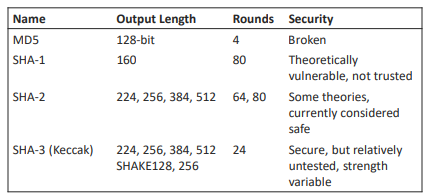
\includegraphics{hash_examples.png}
\end{center}

\section{Message Authentication Codes}
\begin{itemize}
  \item Provide \textit{integrity} and \textit{authenticity}, not confidentiality: protecting system files, ensuring messages haven’t been altered 
  \item Calculate a \textbf{keyed hash} of the message, then \textbf{append this to the end} of the message
\end{itemize}

\subsection{HMAC}
\begin{flushleft}
Double hashing in HMAC handles some weaknesses with traditional MACs.
\end{flushleft}
\begin{center}
  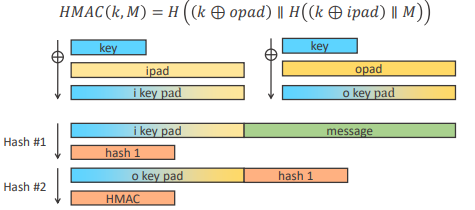
\includegraphics{hmac.png}
\end{center}

\pagebreak
\section*{Reference section} \label{sec:reference}
\begin{description}
	\item[placeholder] \hfill \\
\end{description}
\end{document}
